\documentclass[border=10pt]{standalone}
\usepackage{pgfplots}
\pgfplotsset{compat=1.18}
\begin{document}
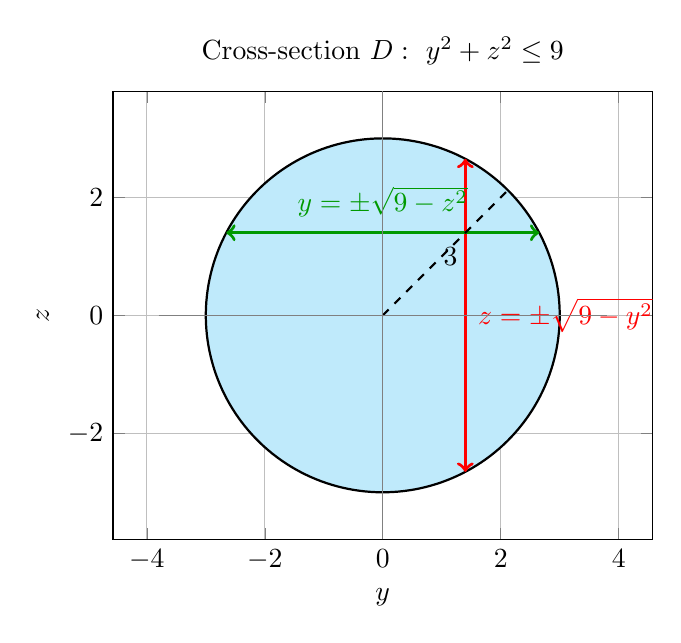
\begin{tikzpicture}
\begin{axis}[
    axis equal,
    xlabel={$y$}, ylabel={$z$},
    xmin=-3.8, xmax=3.8,
    ymin=-3.8, ymax=3.8,
    grid=major,
    title={Cross-section $D:\ y^2+z^2\leq 9$},
    trig format plots=deg,
]
% filled disk
\addplot[fill=cyan!25, draw=black, thick, domain=0:360, samples=200]
({3*cos(x)}, {3*sin(x)}) \closedcycle;

% fixed y = 1.4: z-limits
\draw[<->, red, very thick]
(1.4, {-sqrt(9-1.4^2)}) -- (1.4, {sqrt(9-1.4^2)});
\node[red, right] at (1.45, 0) {$z=\pm\sqrt{9-y^2}$};

% fixed z = 1.4: y-limits
\draw[<->, green!60!black, very thick]
({-sqrt(9-1.4^2)}, 1.4) -- ({sqrt(9-1.4^2)}, 1.4);
\node[green!60!black, above] at (0, 1.5) {$y=\pm\sqrt{9-z^2}$};

% radius 3
\draw[dashed, thick] (0,0) -- ({3*cos(45)}, {3*sin(45)});
\node at (1.15, 1.0) {$3$};

% coordinate axes
\draw[gray] (-3.8,0) -- (3.8,0);
\draw[gray] (0,-3.8) -- (0,3.8);
\end{axis}
\end{tikzpicture}
\end{document}
